\documentclass[12pt,a4paper,ngerman]{article}
\usepackage{stylesheet}
\begin{document}
\TUHeader                          %  Bitte Ausfüllen!!!
%----------------------------
{Übung F: Übertragungsverhalten nachrichtentechnischer Systeme}                       %  Übungstitel
%----------------------------
{25.11.2014}                        %  Übungsdatum
%----------------------------
{05}                            %  Gruppen-Nr.
%----------------------------
{Thomas Neff}                   % Name des Protokollführers
%----------------------------
{
1.~Daniel Freßl, 1230028\\
2.~Thomas Neff, 1230319\\                    %  Übungsteilnehmer
3.~Thomas Pichler, 1230320 \\                   %  ...bei <4 Teilnehmer auskommentieren
4.~Martin Winter, 1130688\\
5.~Bernadette Schreyer, 1073076\\
}
%----------------------------
{Ao.Univ.-Prof. Dipl.-Ing. Dr. techn. Erich Leitgeb}
{Max Henkel}                          %  Betreuer
%----------------------------
{Graz}                              %  Ort der Protokollerstellung
{\today}                            %  Datum Protokollerstellung




\pagebreak
  
\tableofcontents
  
\pagebreak

%-------------------------------------------------------------------------------
%
% Beginn des Protokolls
%
%-------------------------------------------------------------------------------

\section{Demodulation eines QPSK-Signals mit unbekannten Paramteren}
\subsection{Aufgabenstellung}
Gegeben ist ein Signal, welches mittels QPSK auf einen HF-Träger moduliert wurde. Sie sollen dieses Signal nun mit dem in der Software integrierten digitalen Demodulator demodulieren. Da Ihnen die Paramter Trägerfrequenz, Symbolrate und senderseitig verwendetes Filter unbekannt sind, müssen Sie diese bestimmen.
\begin{itemize}
\item Bestimmen Sie die Trägerfrequenz und stellen Sie das Signal in Frequenz- und Zeitbereich sinnvoll dar. 
\item Bestimmen Sie die Symbolrate. Versuchen Sie dazu die Darstellung des Spektrums zu glätten.
\item Bestimmen Sie anhand des Spektrums den Filtertyp und dessen Parameter.
\item Demodulieren Sie das Signal. Stellen Sie Konstellations- und Augendiagramm sowie das Spektrum des Signals dar. 
\item Woran ist erkennbar, dass der richtige Filtertyp gefunden wurde. Überprüfen Sie ihre Antwort durch Veränderung der Einstellungen
\end{itemize}
\subsection{Messaufbau}
Das zu analysierende Signal wurde mit einem Vektorsignalgenerator generiert und mit dem Oszilloskop für die Analyse digitalisiert.  
\subsection{Tabellen}
Es waren keine Tabellen aufzunehmen. 
\subsection{Formeln}
Die Formel für die Nyquist-Frequenz lautet
\begin{equation}
f_N = \frac{f_S}{2}
\end{equation}
Die absolute Bandbreite ergibt sich durch
\begin{equation}
B = B_N (1+\alpha)
\end{equation}
\subsection{Berechnungsbeispiele}
\pagebreak
\subsection{Diagramme}
\begin{figure}[H]
\centering
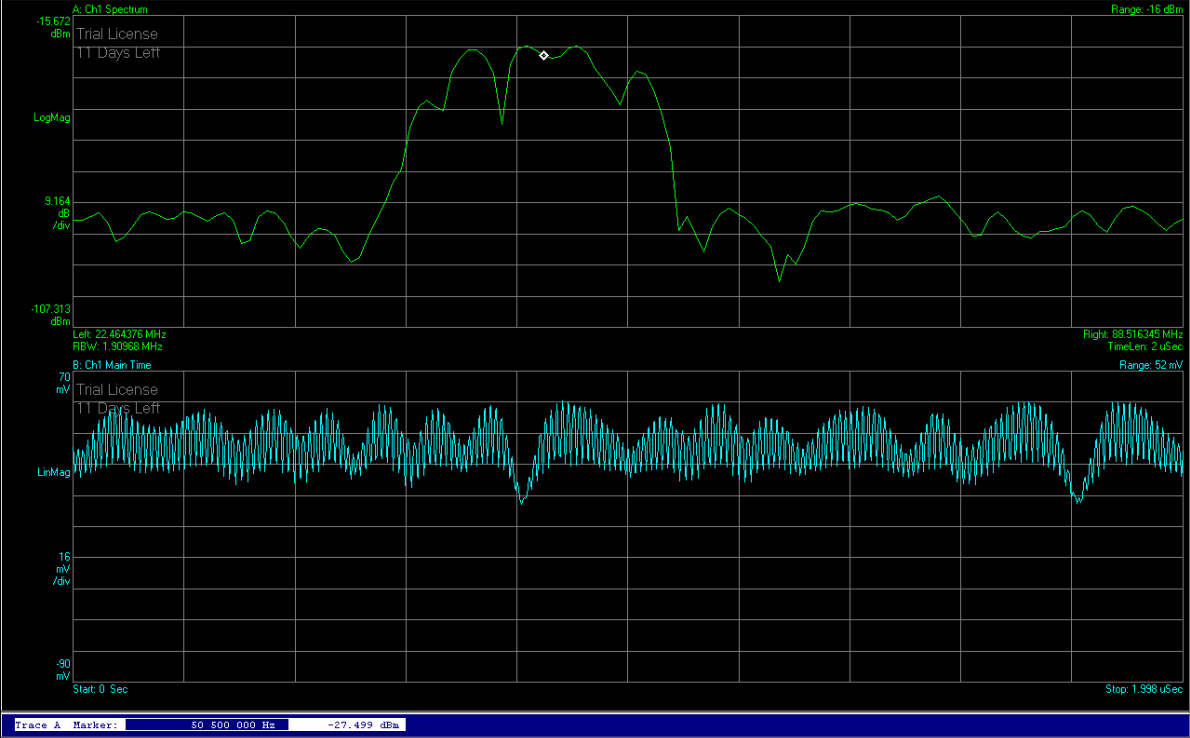
\includegraphics[width=0.9\textwidth]{figures/Aufgabe1_QPSK.jpg} 
\caption{Signal in Frequenz- und Zeitbereich}
\end{figure}


\begin{figure}[H]
\centering
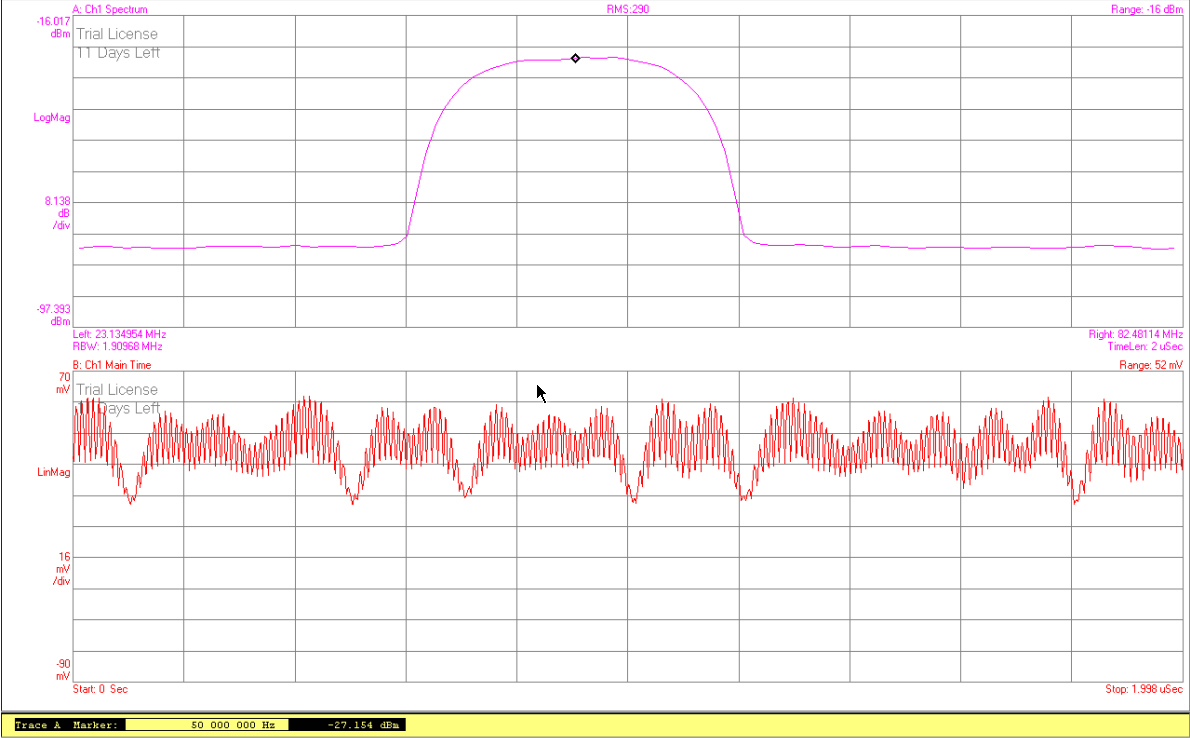
\includegraphics[width=0.9\textwidth]{figures/Aufgabe1_QPSK_avg.jpg} 
\caption{Signal gemittelt in Frequenz- und Zeitbereich}
\end{figure}

\pagebreak

\begin{figure}[H]
\centering
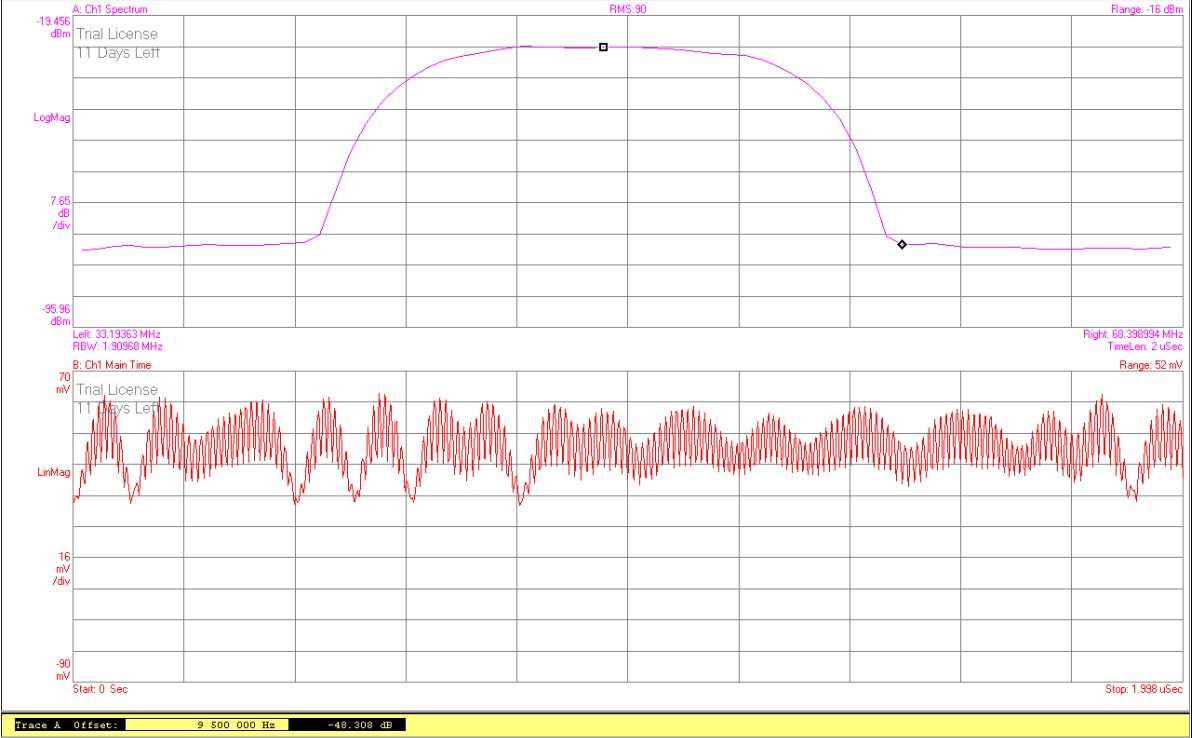
\includegraphics[width=0.9\textwidth]{figures/Aufgabe1_QPSK_B.jpg} 
\caption{Ermittlung von $f_N$ mittels Marker}
\end{figure}

\begin{figure}[H]
\centering
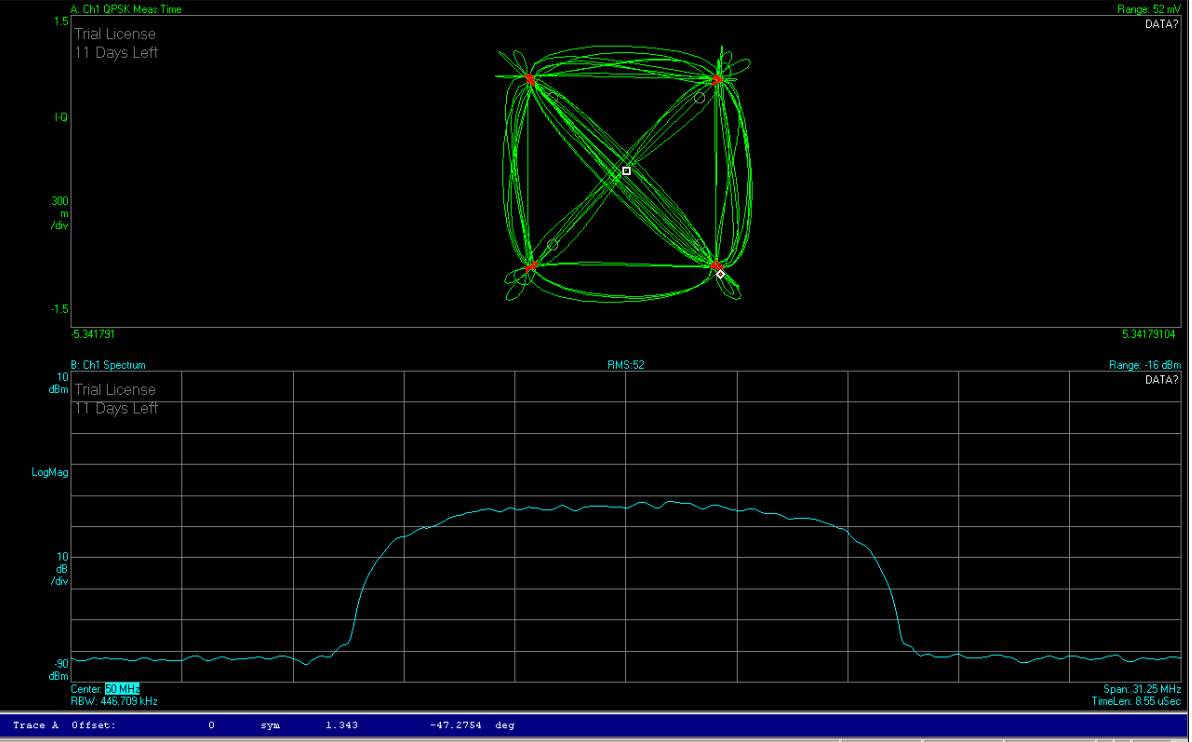
\includegraphics[width=0.9\textwidth]{figures/Aufgabe1_QPSK_demod.jpg} 
\caption{Konstellationsdiagramm des Signals}
\end{figure}

\pagebreak

\begin{figure}[H]
\centering
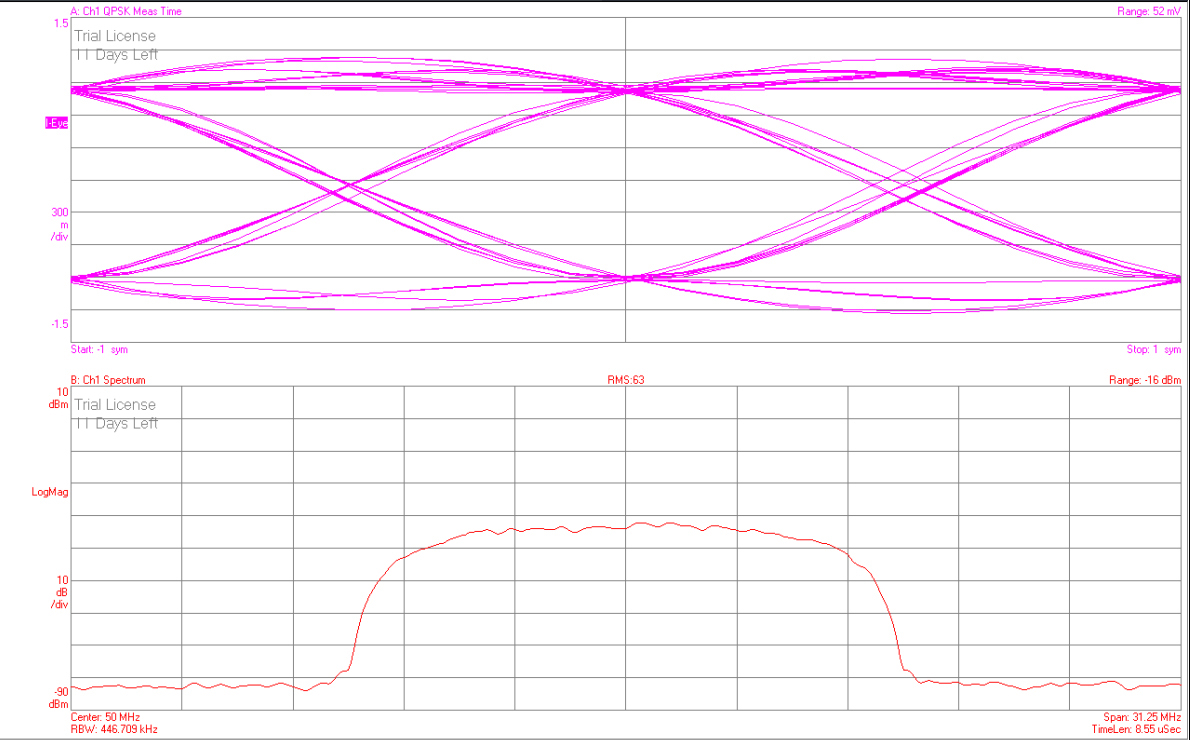
\includegraphics[width=0.9\textwidth]{figures/Aufgabe1_QPSK_demod_i_eye.jpg} 
\caption{Augendiagramm des Signals}
\end{figure}

\begin{figure}[H]
\centering
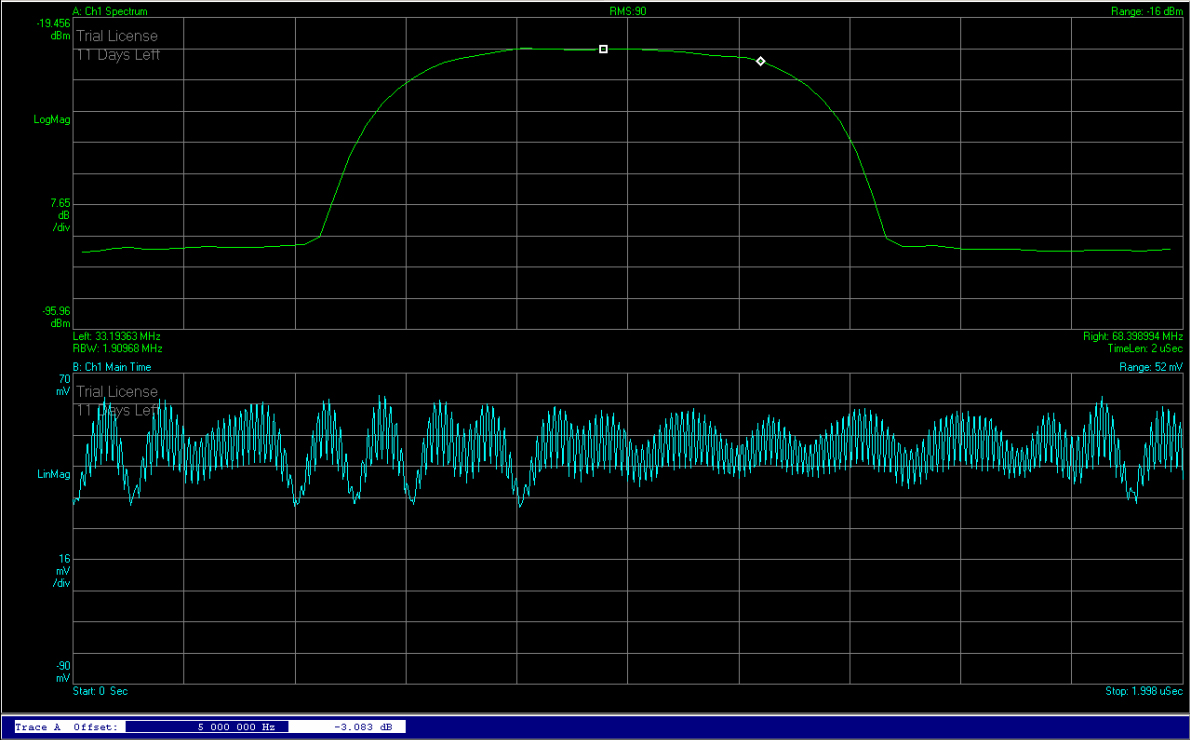
\includegraphics[width=0.9\textwidth]{figures/Aufgabe1_QPSK_fs.jpg} 
\caption{Test}
\end{figure}
\pagebreak

\subsection{Diskussion}
\begin{enumerate}
\item Trägerfrequenz: $50MHz$
\item $f_N = \frac{f_S}{2} \Rightarrow f_S = 2 \cdot f_N$, Differenz $5 MHz = f_N \Rightarrow f_S = 2 \cdot f_N = 10 MHz$
\item RC- Filter. $B = B_N (1 + \alpha) B = 19Mhz \quad B_N = 10 MHz \Rightarrow \alpha = 0.9$
\item Symbolrate = 10MHz Format: QPSK
\end{enumerate}
Aus Augendiagramm erkennbar, Linien sauber in einem Punkt geschnitten


\pagebreak



\section{Kanalverzerrungen / Equalizer}
\subsection{Aufgabenstellung}
Ein mittels 16-QAM moduliertes breitbandiges Signal wird über einen nicht-idealen Kanal mit Bandbegrenzung übertragen. Es sollen die entstandenen Verzerrungen mit einem Equalizer entfernt werden. Weiters soll die Übertragunsfunktion des Kanals dargestellt werden. 
\begin{itemize}
\item Beurteilen Sie die Verzerrungen anhand des Spektrums.
\item Versuchen Sie, das verzerrte 16-QAM-Signal zu demodulieren. Stellen Sie Augen- und Konstellationsdiagramm dar. Beurteilen Sie anhand dieser Darstellungen die Signalqualität (beachten Sie auch Kenngrößen wie EVM und MER).
\item Wenden Sie einen Equalizer an, um die Verzerrungen zu beseitigen. Wählen Sie dabei verschiedene Darstellungsmöglichkeiten, mit denen Sie die Verbesserung der Signalqualität belegen können. 
\item Stelle Sie die Übertragungsfunktion des Kanals dar. 
\end{itemize}
\cite[18]{skript}

\subsection{Messaufbau}
Es wurde kein Messaufbau benötigt.
\subsection{Tabellen}
Es waren keine Tabellen aufzunehmen. 
\subsection{Formeln}
Es wurden keine Formeln benötigt.
\subsection{Berechnungsbeispiele}
Es wurden keine Berechnungen durchgeführt.

\pagebreak
\subsection{Diagramme}
\begin{figure}[H]
\centering
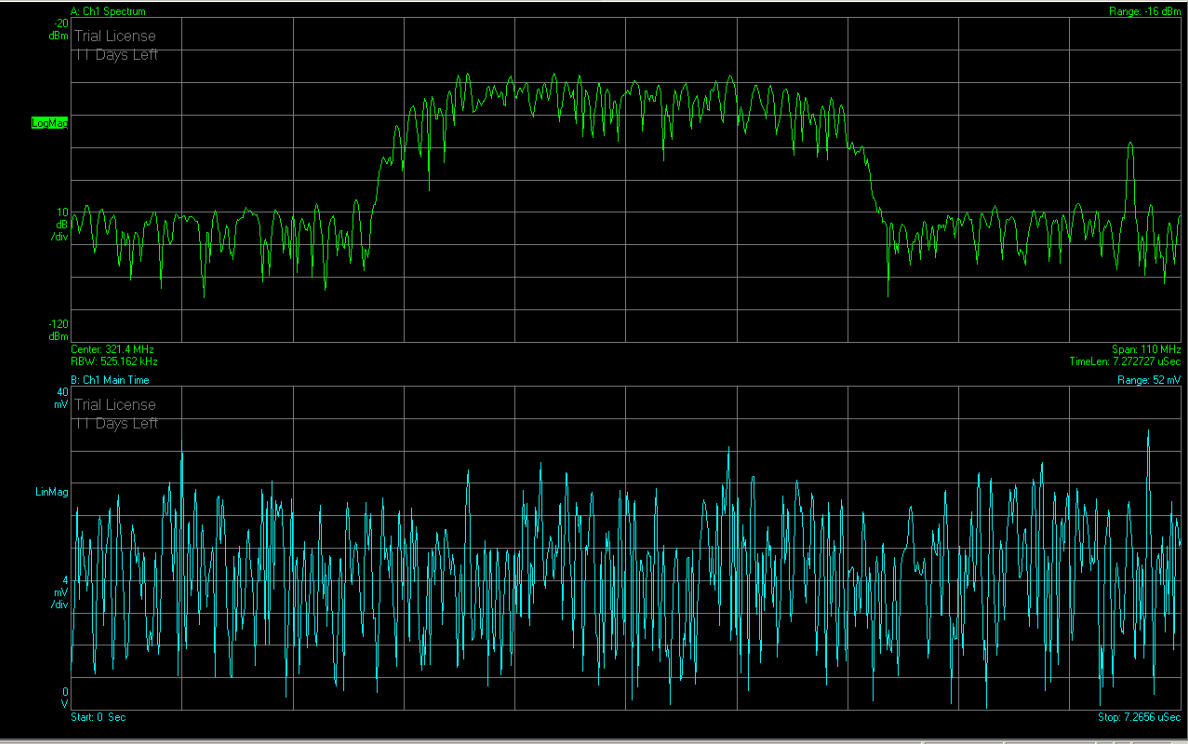
\includegraphics[width=0.9\textwidth]{figures/Aufgabe2_16QAM_1.jpg} 
\caption{Spektrum und zeitlicher Verlauf des empfangenen 16-QAM modulierten Signals}\label{fig:aufg2_16QAM_spec}
\end{figure}

\begin{figure}[H]
\centering
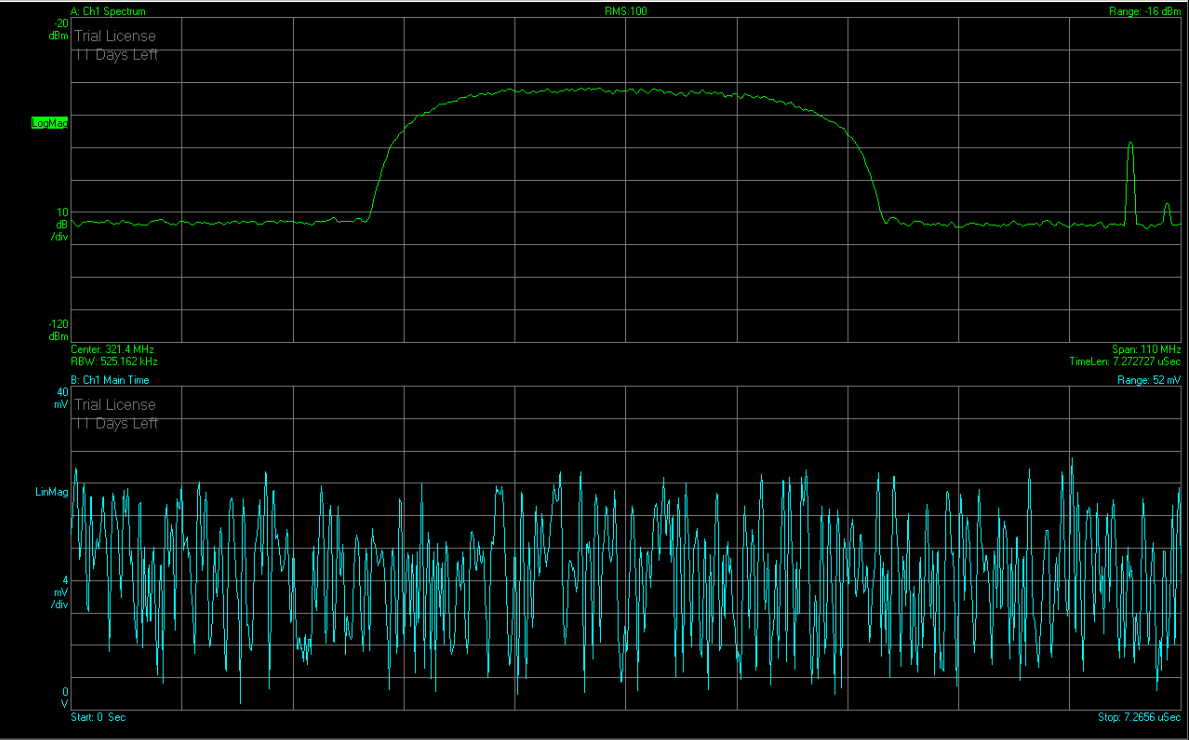
\includegraphics[width=0.9\textwidth]{figures/Aufgabe2_16QAM_avg.jpg} 
\caption{Spektrum und zeitlicher Verlauf des Signals nach dem Glätten.}\label{fig:aufg2_16QAM_spec_avg}
\end{figure}

\pagebreak
\begin{figure}[H]
\centering
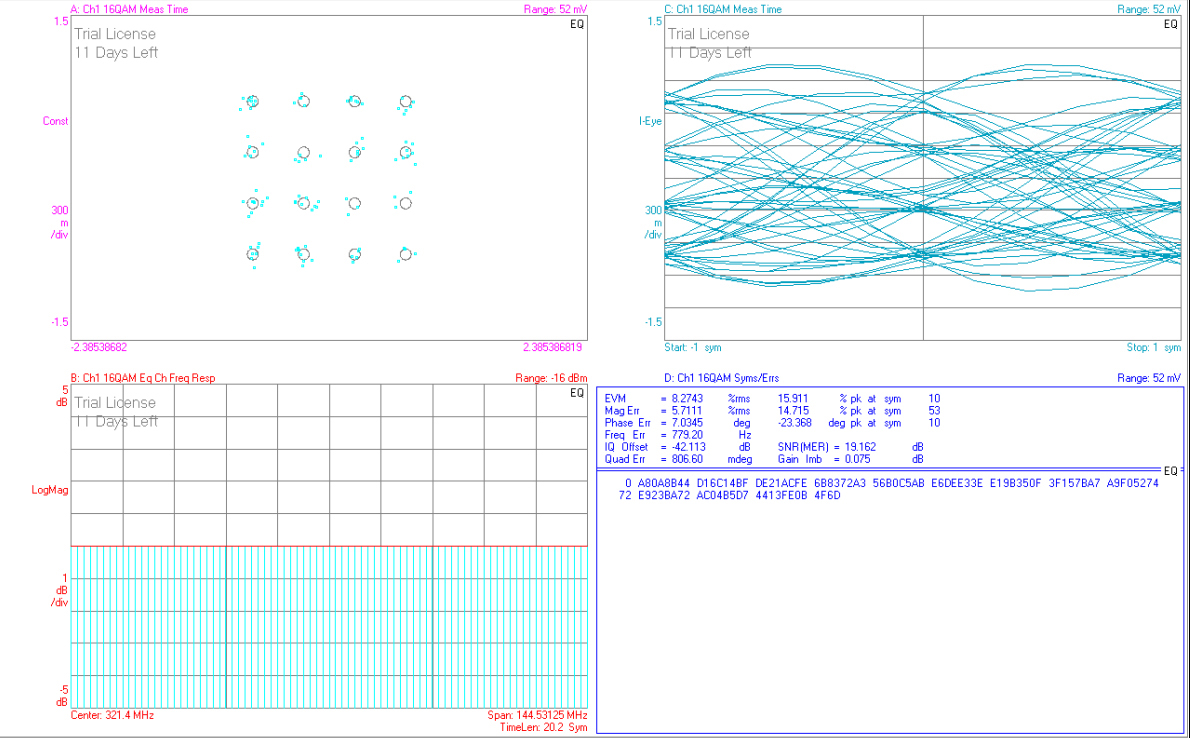
\includegraphics[width=0.9\textwidth]{figures/Aufgabe3_16QAM_demod.jpg} 
\caption{Konstellations- und Augendiagramm des Signals, weiters Amplitudenfrequenzgang des Equalizer und Kanals und Kennwerte zur Beurteilung der Signalqualität}\label{fig:aufg2_16QAM_demod}
\end{figure}

\begin{figure}[H]
\centering
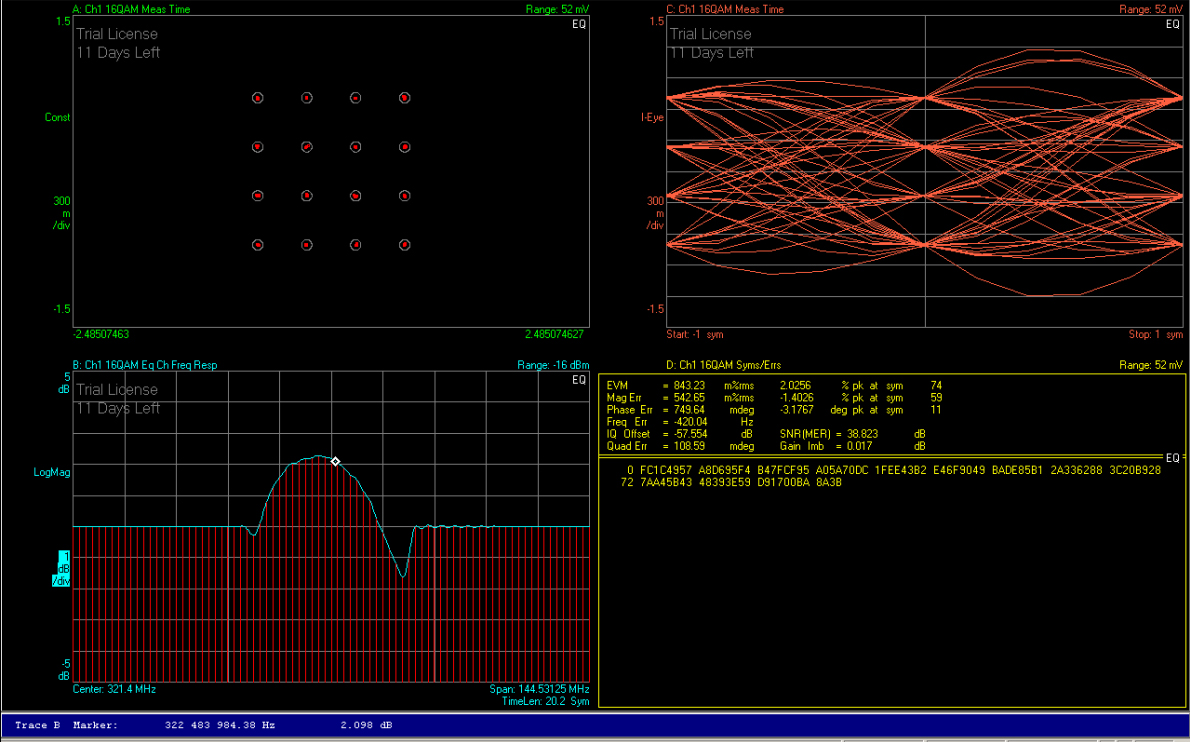
\includegraphics[width=0.9\textwidth]{figures/Aufgabe2_16QAM_demod_equal.jpg} 
\caption{Darstellung wie in Abbildung \ref{fig:aufg2_16QAM_demod}. Im Amplitudenfrequenzgang ist die Anpassung durch den Equalizer zu sehen. }\label{fig:aufg2_16QAM_demod_equal}
\end{figure}


\subsection{Diskussion}
Bei dieser Aufgabenstellung wurden bereitgestellte Daten (breitbandiges Signal), welche laut Aufgabenstellung mittels 16-QAM moduliert und über einen nicht-idealen Kanal mit Bandbegrenzung übertragen worden sind und die entsprechende Konfiguration in die Software \emph{Agilent 89600 Vector Signal Analysis Software} geladen.\\
Wie in Abbildung \ref{fig:aufg2_16QAM_spec} zu sehen, war das Spektrum ziemlich verrauscht. Um das Spektrum leichter interpretieren zu können wurde das Signal mit der Software und den Einstellungen \emph{Average Type RMS (Video)} und \emph{Count 100} geglättet.\\
In Abbildung \ref{fig:aufg2_16QAM_spec_avg}, in der das geglättete Spektrum zu sehen ist, erkennt man das die Frequenzen über der Mittenfrequenz (321,4 MHz) mehr gedämpft werden als niedrigere Frequenzen. Weiters treten bei ungefähr 370Mhz und 375MHz hochfrequente Störungen auf, welche herausgefilter werden sollten (mittels Filter im Demodulator).\\
Die ungleiche Dämpfung der verschiedenen Frequenzanteile des Signals sind Verzerrungen die durch den nicht-idealen Kanal verursacht werden.\\
\\
Zur demodulation wurde eine andere Konfiguration geladen.
\begin{enumerate}
\item EVM und MagErr aus Bild auslesen.
\end{enumerate}


\pagebreak



\section{Vergleich digitaler Phasenmodulationsverfahren}
\subsection{Aufgabenstellung}
Gegeben ist eine Reihe von Signalen, welche mit unterschiedlichen digitalen Phasenmodulationsverfahren moduliert wurden (QPSK, $\pi/4$-DQPSK, OQPSK, MSK und GMSK). Da es sich um Phasenmodulationsverfahren handelt, sollte die Hüllkurve dieser Signale idealerweise konstant sein. Speziell bei QPSK gibt es aber mitunter starke Einbrüche in der Hüllkurve. Sie sollen nun eine Reihe von Modualtionsverfahren auf ihre Eigenschaften untersuchen. 
\begin{itemize}
\item Demodulieren Sie die Signale und beurteilen Sie die Übergänge zwischen den Symbolen. Diskutieren Sie den Einfluss dieser Übergänge auf die Hüllkurve. 
\item Stellen Sie den Phasenverlauf dar und diskutieren Sie diesen.
\item Finden Sie einen alternativen Weg, Aussagen über die Hüllkurvenschwankungen treffen zu können.
\end{itemize}


\subsection{Tabellen}
Es waren keine Tabellen aufzunehmen. 
\subsection{Formeln}

\subsection{Berechnungsbeispiele}


\pagebreak
\subsection{Diagramme}
\begin{figure}[H]
\centering
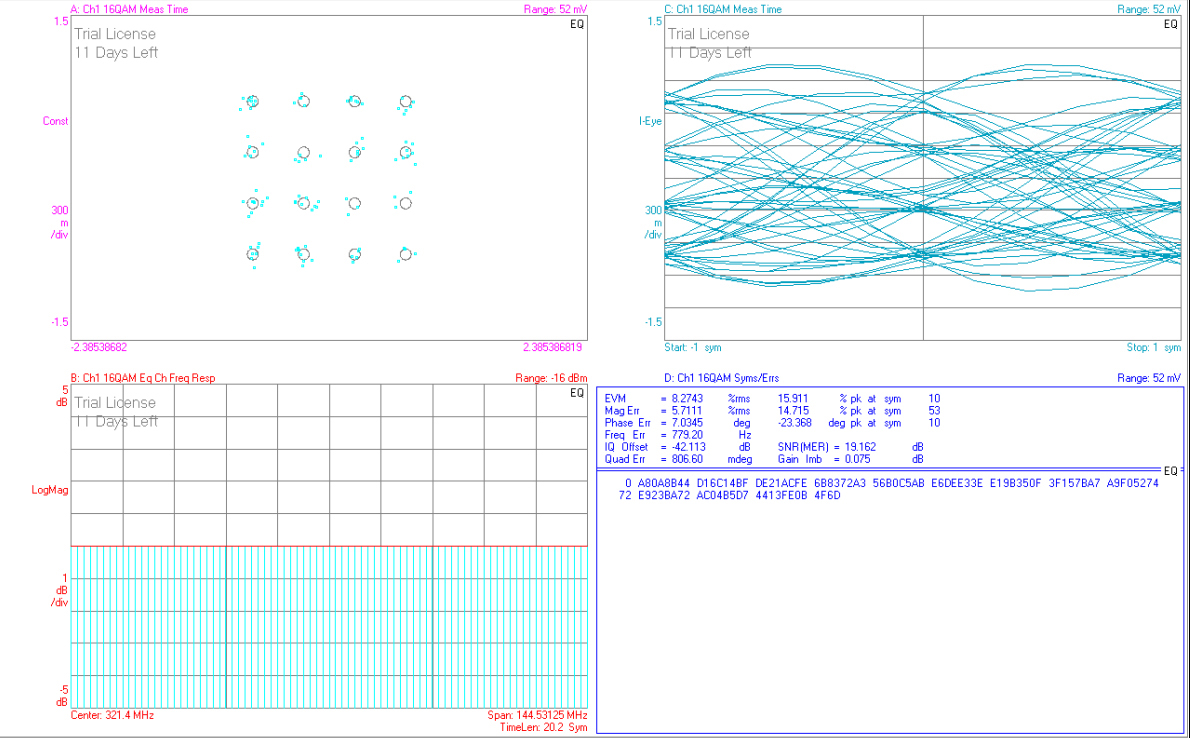
\includegraphics[width=0.9\textwidth]{figures/Aufgabe3_16QAM_demod.jpg} 
\caption{Test}
\end{figure}

\begin{figure}[H]
\centering
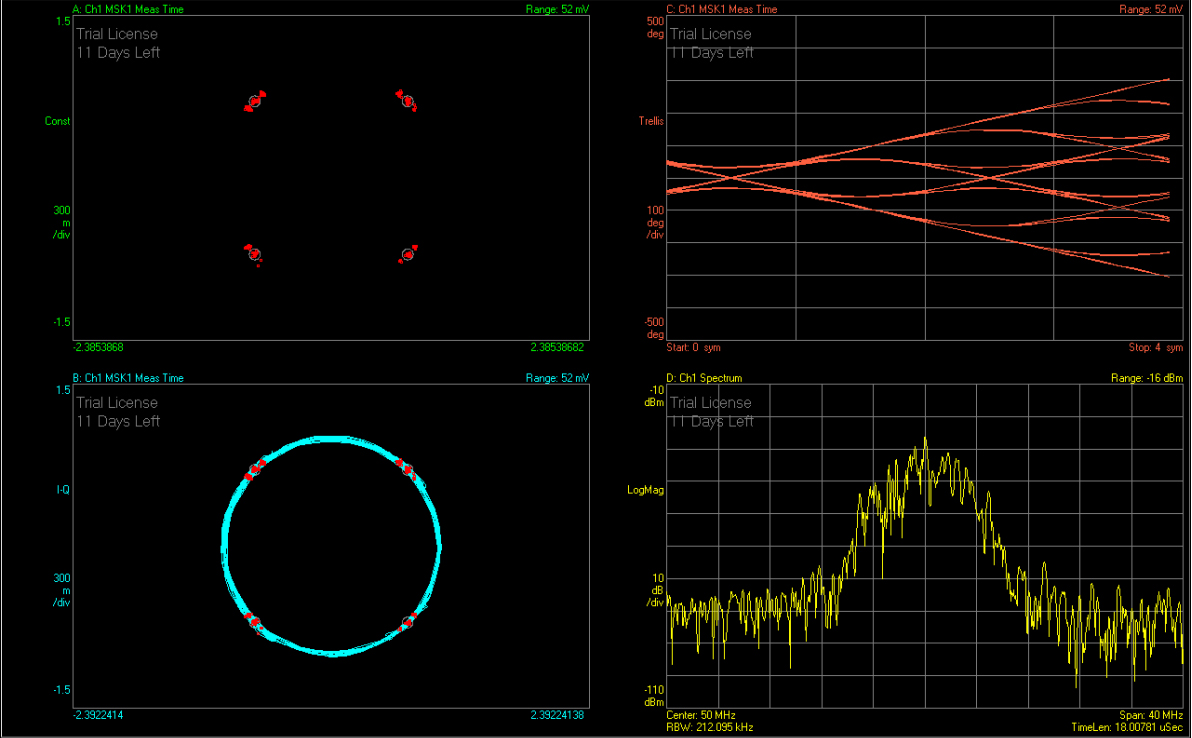
\includegraphics[width=0.9\textwidth]{figures/Aufgabe3_GMSK.jpg} 
\caption{Test}
\end{figure}


\pagebreak
\begin{figure}[H]
\centering
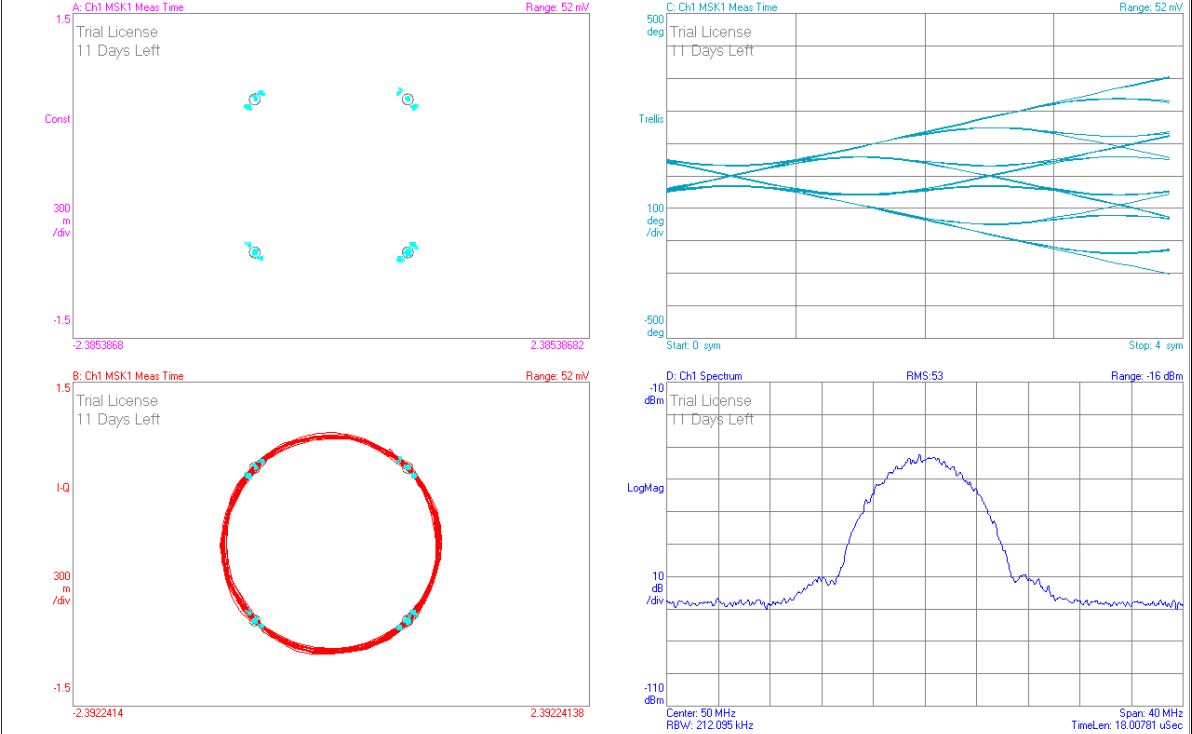
\includegraphics[width=0.9\textwidth]{figures/Aufgabe3_GMSK_avg.jpg} 
\caption{Test}
\end{figure}

\begin{figure}[H]
\centering
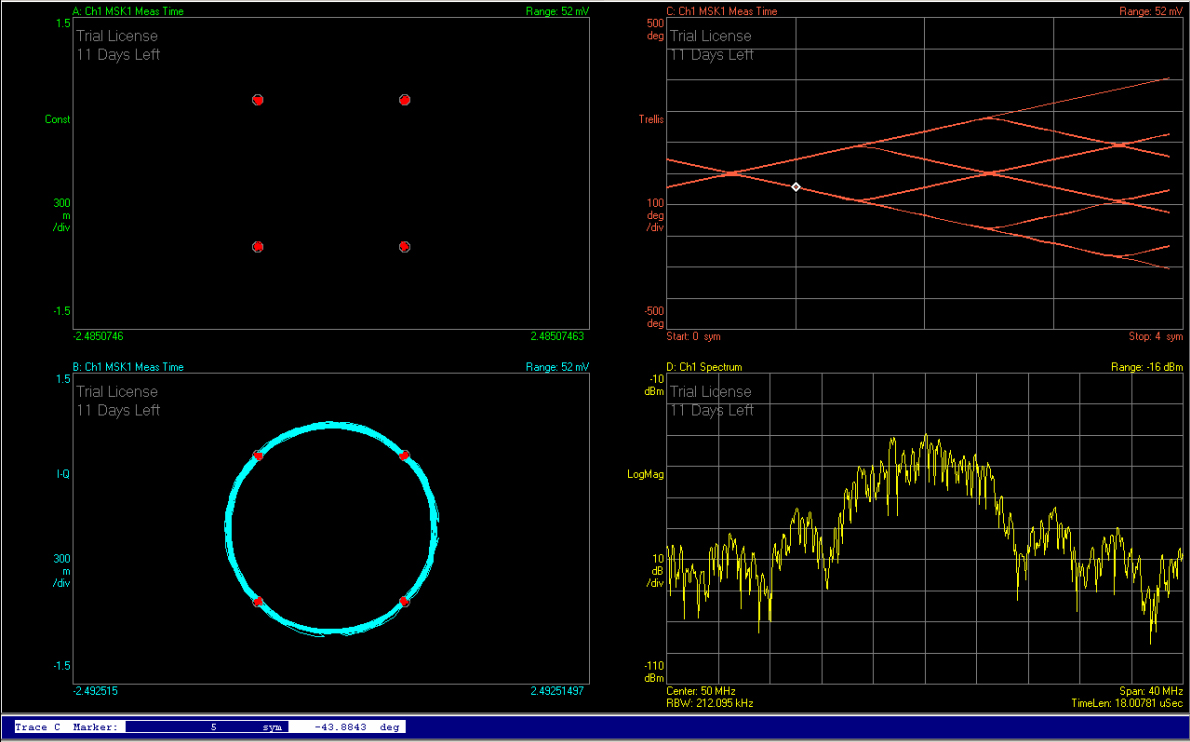
\includegraphics[width=0.9\textwidth]{figures/Aufgabe3_MSK.jpg} 
\caption{Test}
\end{figure}


\pagebreak
\begin{figure}[H]
\centering
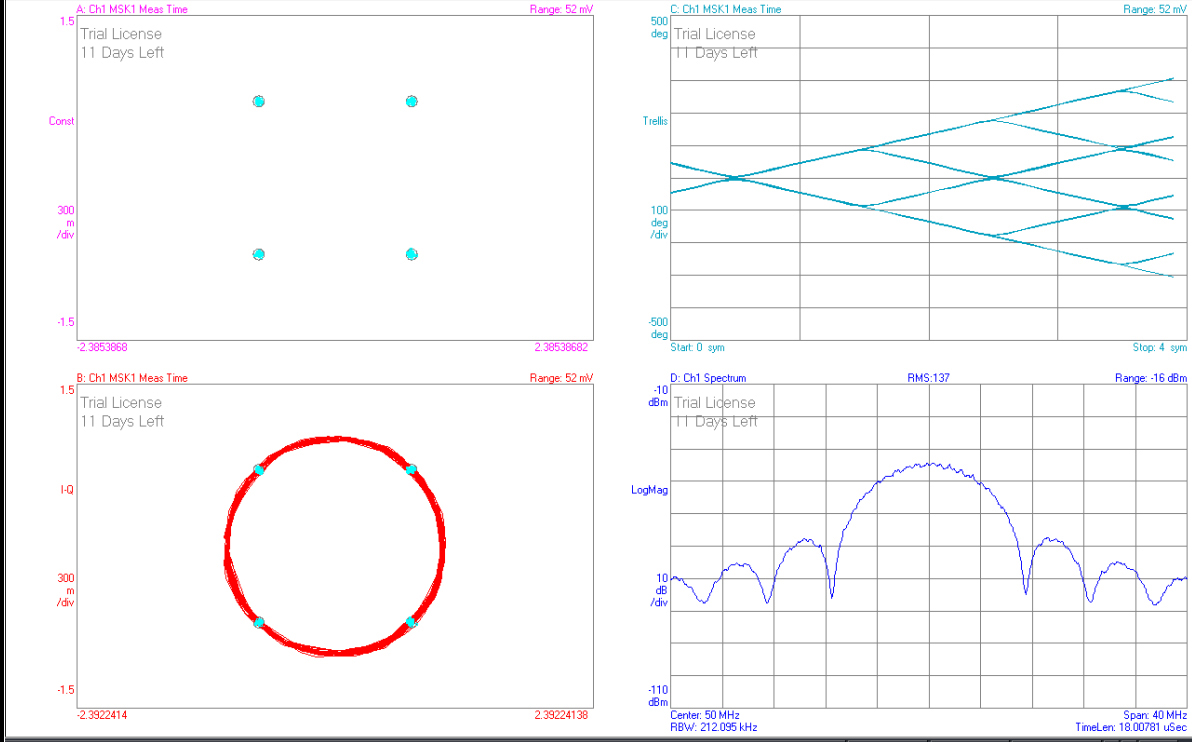
\includegraphics[width=0.9\textwidth]{figures/Aufgabe3_MSK_avg.jpg} 
\caption{Test}
\end{figure}

\begin{figure}[H]
\centering
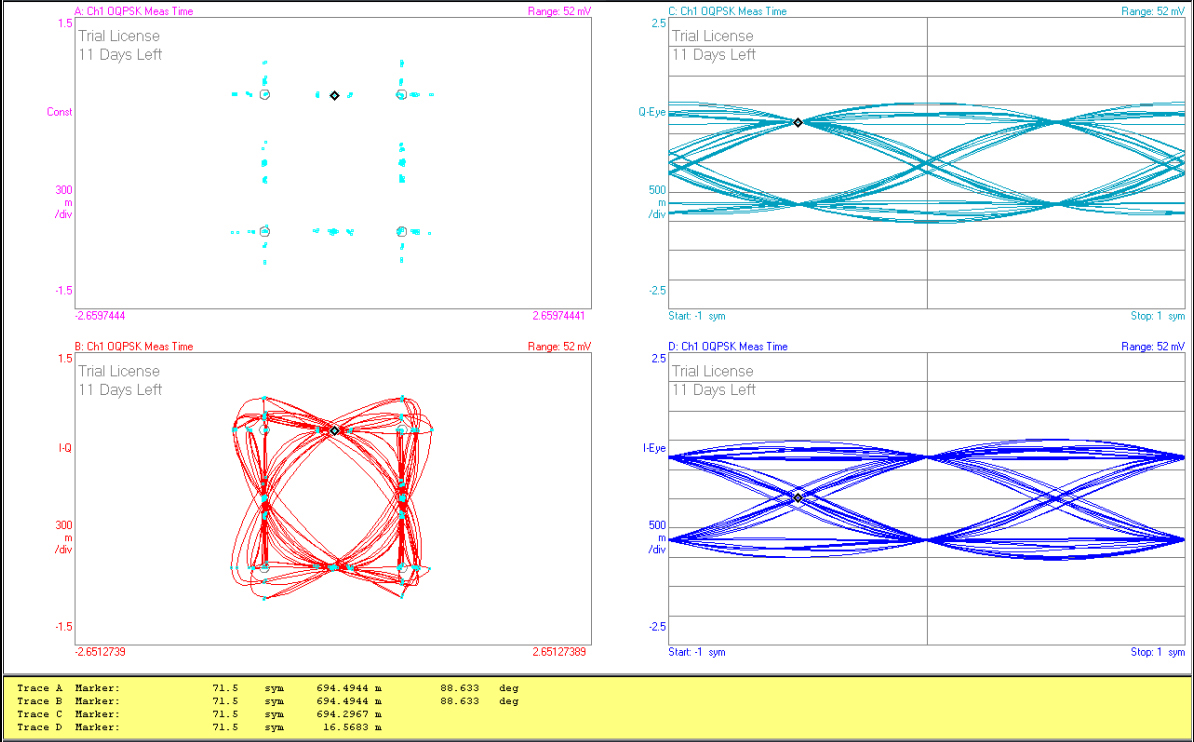
\includegraphics[width=0.9\textwidth]{figures/Aufgabe3_OQPSK.jpg} 
\caption{Test}
\end{figure}


\pagebreak
\begin{figure}[H]
\centering
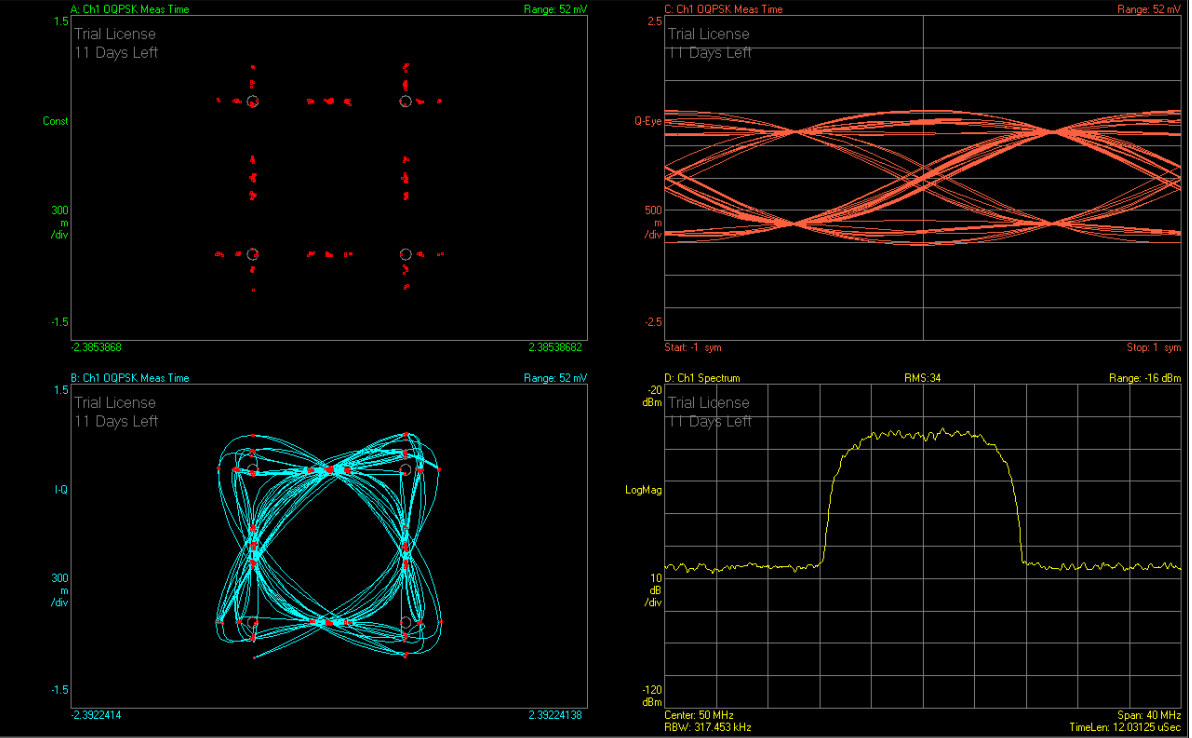
\includegraphics[width=0.9\textwidth]{figures/Aufgabe3_OQPSK_avg.jpg} 
\caption{Test}
\end{figure}

\begin{figure}[H]
\centering
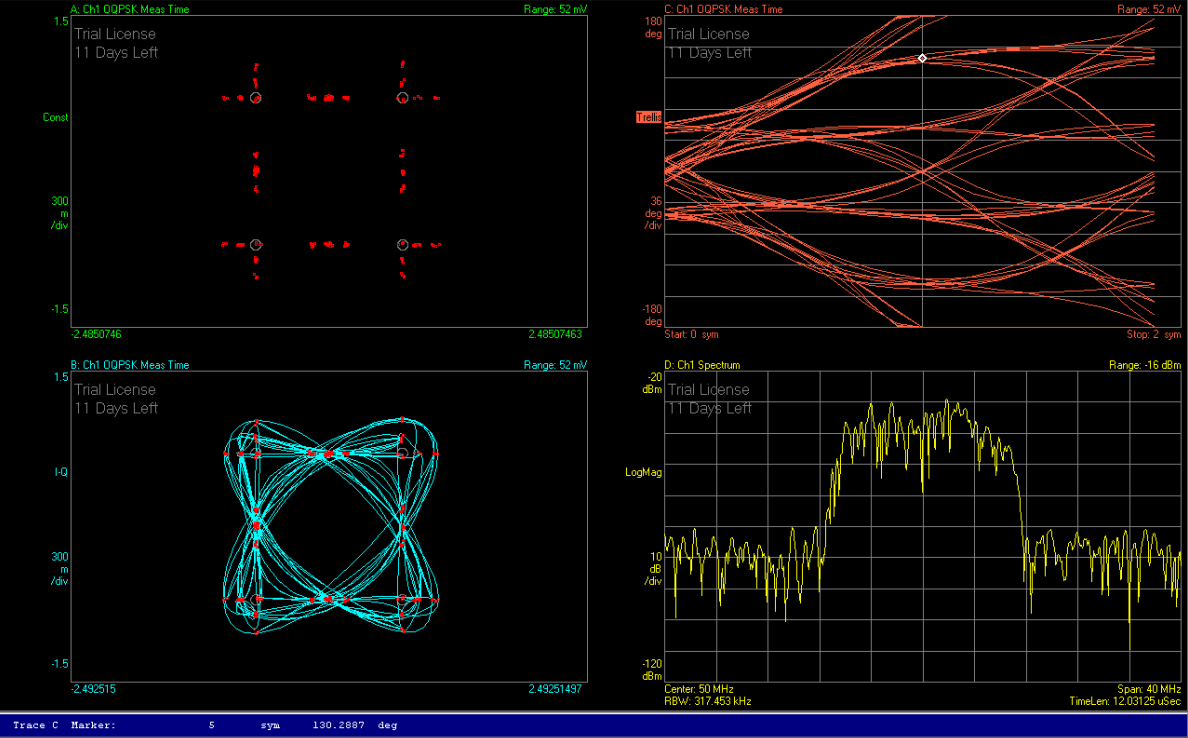
\includegraphics[width=0.9\textwidth]{figures/Aufgabe3_OQPSK_phase.jpg} 
\caption{Test}
\end{figure}


\pagebreak
\begin{figure}[H]
\centering
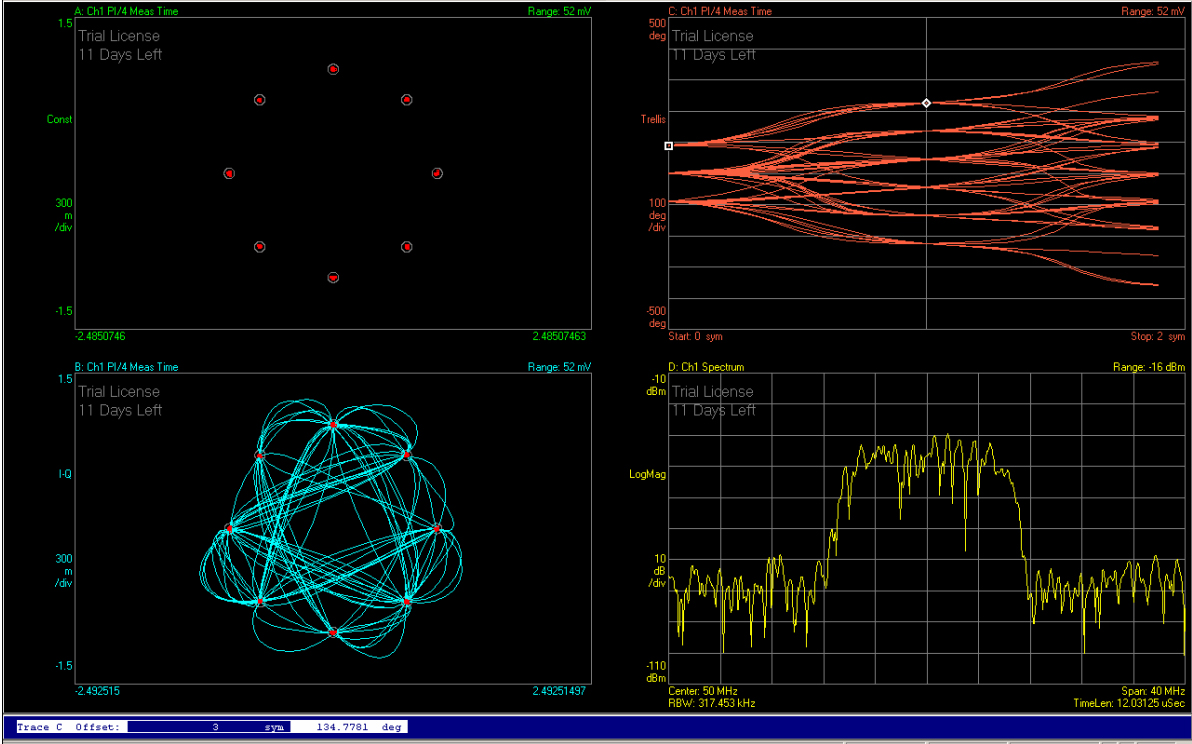
\includegraphics[width=0.9\textwidth]{figures/Aufgabe3_pi4DQPSK.jpg} 
\caption{Test}
\end{figure}

\begin{figure}[H]
\centering
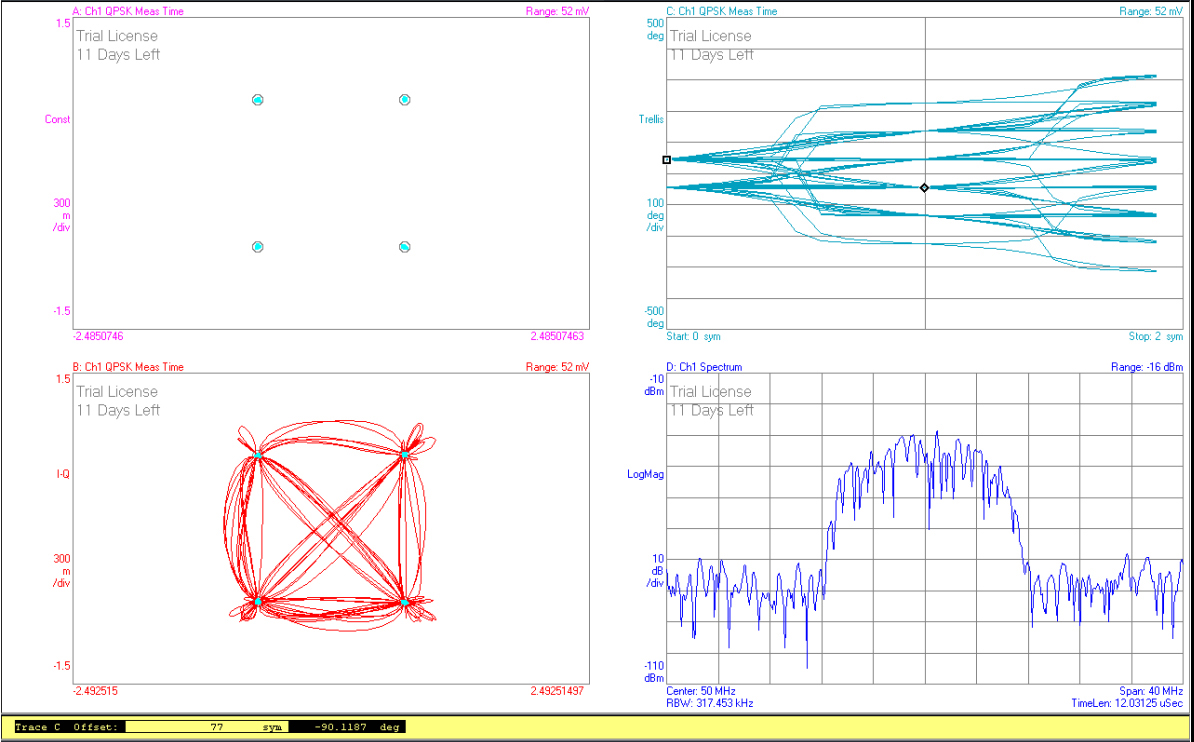
\includegraphics[width=0.9\textwidth]{figures/Aufgabe3_QPSK.jpg} 
\caption{Test}
\end{figure}

\pagebreak

\subsection{Diskussion}
OQPSK - Abtastzeitpunkt führt zu der Darstellung, Q-Phase wird genau zwischen zwei idealen Zeitpunkten abgetastet. 


\pagebreak



\section{GSM}
\subsection{Aufgabenstellung}
Gegeben ist eine 65ms lange Aufzeichnung aus dem Frequenzbereich von 930-960MHz (oberer Bereich des Downlinks bei GSM 900). Sie sollen in diesem Bereich verschiedene GSM-Kanäle beobachten und ein möglichst starkes Signal demodulieren. Hierzu müssen Sie aufgrund des geringen SNR auf eine genaue Einstellung des Demodulators und des verwendeten Messbereichs achten. 
\begin{itemize}
\item Visualisieren Sie den gegebenen Frequenzbereich mittels Spektrogramm. Suchen Sie einen Kanal, welcher Ihnen zur Untersuchung geeignet erscheint.
\item Versuchen Sie, im Zeitbereich einen Burst zu finden. Versuchen Sie, die GSM Framestruktur zu visualisieren.
\item Stellen Sie den digitalen Demodulator auf die Parameter von GSM ein. Stellen Sie Spektrum, Konstellationsdiagramm und Zeitbereich dar. Diskutieren Sie auch den Phasenverlauf. 
\item Diskutieren Sie die im Skriptum angeführten Parameter von GSM anhand von Spektrum, Spektrogramm, Zeitbereich und digitalem Demodulator. 
\end{itemize}

\subsection{Messaufbau}
Der Messaufbau ähnelt dem von Übung 2, wobei das Signal hier aber nicht generiert, sondern über eine Antenne empfangen wurde. Das wiederum auf $321.4$MHz transformierte Signal wird dem Oszilloskop zur Digitalisierung zugeführt. 
\subsection{Tabellen}
Es waren keine Tabellen aufzunehmen. 
\subsection{Formeln}

\subsection{Berechnungsbeispiele}
\pagebreak
\subsection{Diagramme}
\begin{figure}[H]
\centering
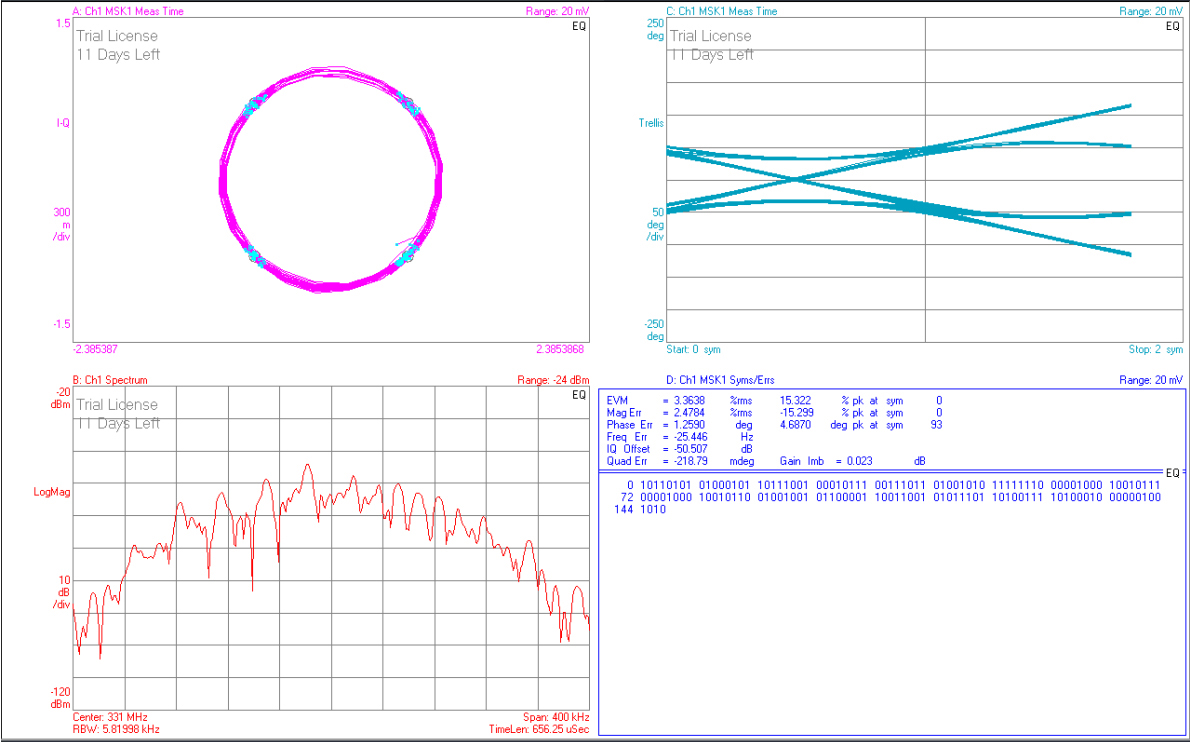
\includegraphics[width=0.9\textwidth]{figures/Aufgabe4_demod.jpg} 
\caption{Test}
\label{fig:a4demod}
\end{figure}

\begin{figure}[H]
\centering
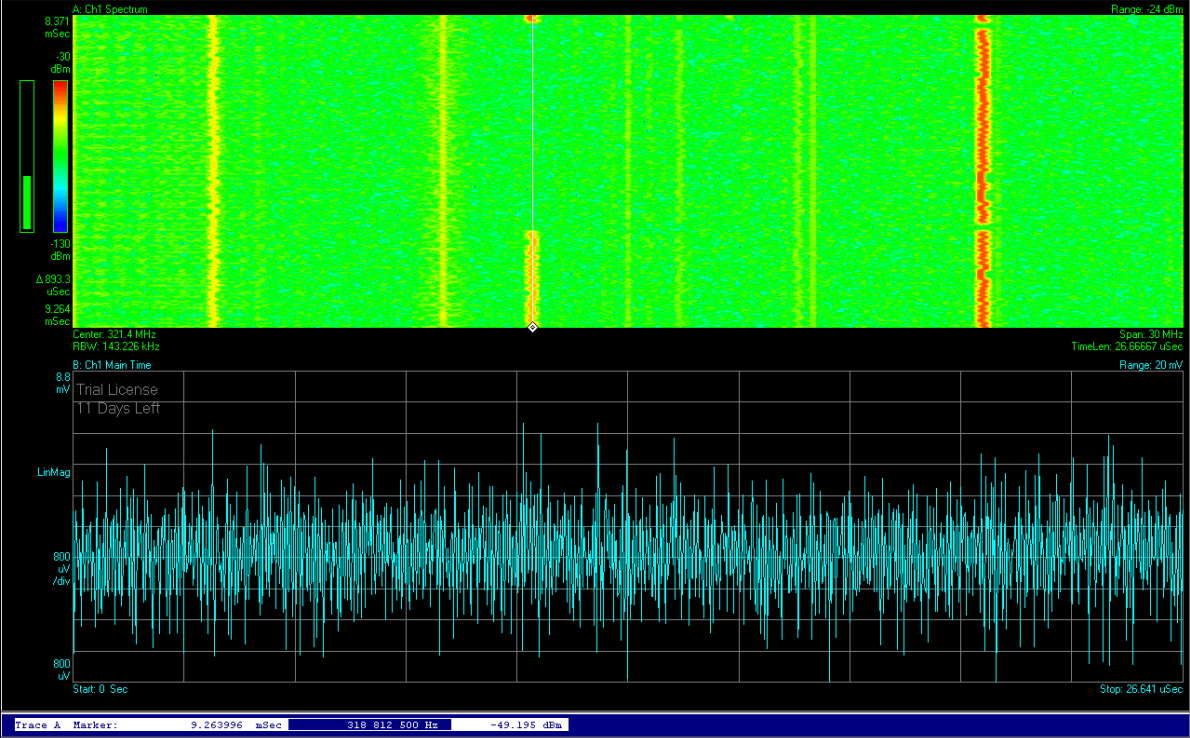
\includegraphics[width=0.9\textwidth]{figures/Aufgabe4_Spektrogramm.jpg} 
\caption{Test}
\label{fig:spectrogram}
\end{figure}




\subsection{Diskussion}

Im Spektrogramm (Abbildung: \ref{fig:spectrogram}) sind recht deutlich die verschiiedenen Kanäle, die auf verschiedene Frequenzen aufgeteilt sind, zu erkennen. Zur Bestimmung der Länge eines Bursts haben wir das Spektrogramm im richtigen Zeitpunkt angehalten. Unsere Messung lieferte als Länge eines Frame-Bursts bei GSM $\approx 800 \mu S$. 

Außerdem ist ersichtlich, dass zwischen den einzelnen Bursts Pausen (Guard Periods) im Spektrogramm sind. Diese sind dazu da, dass es zwischen Übertragungen keine Überschneidungen gibt, da es sonst zu Datenverlust führen würde. Die Guard Periods haben eine zeitliche Dauer von $\approx 30 \mu S$.

Entsprechend der Theorie sollte ein Burst eine Dauer von $576.92 \mu S$ (inklusive Guard Period) besitzen. Der Unterschied ist dadurch zu erklären, dass unsere Methode zur Messung (Spektrogramm anzeigen und im richtigen Zeitpunkt anhalten) sehr ungenau ist.

Der Phasenverlauf von GSM aus Abbildung \ref{fig:a4demod} weist keine Knicke oder Unstetigkeiten auf. Zwischen den Symbolen ändert sich die Phase also stetig, so wie es bei GMSK (Gaussian Minimum Shift Keying) sein sollte. Das Konstellationsdiagramm zeigt, dass die Amplitude der Hüllkurve konstant bleibt, da die Amplitude jedes Symbols gleich groß ist (Radius vom Kreis ist konstant).

Das Frequenzspektrum zeigt eine Mittenfrequenz von $331 MHz$ und eine Spanne von $400 kHz$. Aus der Theorie ist bekannt, dass ein Frequenzkanal bei GSM eine Bandbreite von $200 kHz$ besitzt. Im Spektrum aus Abbildung \ref{fig:a4demod} sieht man sehr gut, dass man mit dem verwendeten Modulationsverfahren (GMSK) auch noch Signaleinstreuungen (Adjacent Channel Interference) nach der Bandbreite von $200 kHz$ hat. Deswegen ist zwischen jedem $200 kHz$ Band bei GSM noch ein Guard Band mit einer Bandbreite von $100 kHz$ um das Übersprechen auf einen benachbarten Kanal gering zu halten.

Standardisierte Trägerfrequenzen / Mittenfrequenzen für GSM sind laut Skriptum bei $900 MHz$ bzw. $1800 MHz$. Für unser Messsystem wurde anscheinend keine Standardisierte Trägerfrequenz verwendet.

DIGITALER MODULATOR???? Keine Ahnung mehr.



\begin{thebibliography}{9}

\bibitem{skript}
  Markus Lenzhofer, Paul Meissner, Dr. Klaus Witrisal.
  \emph{Übung E: Messungen an digitalen Übertragungssystemen}.
  Technische Universität Graz.

\end{thebibliography}


 



   
\end{document}